
\documentclass[12pt]{article}

\usepackage{xcolor}
\usepackage{tcolorbox}
\usepackage[colorlinks=true]{hyperref}
\usepackage{verbatim}
\usepackage[margin=1.5cm]{geometry}
\usepackage{natbib}

\newenvironment{instruction}{%
    \begin{tcolorbox}[colback=red!5,colframe=red,title=Instruction]%
}{%
    \end{tcolorbox}%
}


\usepackage{titlesec}
% begin add subsubsubsection
\titleclass{\subsubsubsection}{straight}[\subsection]

\newcounter{subsubsubsection}[subsubsection]
\renewcommand\thesubsubsubsection{\thesubsubsection.\arabic{subsubsubsection}}
\renewcommand\theparagraph{\thesubsubsubsection.\arabic{paragraph}} % optional; useful if paragraphs are to be numbered

\titleformat{\subsubsubsection}
  {\normalfont\normalsize\bfseries}{\thesubsubsubsection}{1em}{}
\titlespacing*{\subsubsubsection}
{0pt}{3.25ex plus 1ex minus .2ex}{1.5ex plus .2ex}

\makeatletter
\renewcommand\paragraph{\@startsection{paragraph}{5}{\z@}%
  {3.25ex \@plus1ex \@minus.2ex}%
  {-1em}%
  {\normalfont\normalsize\bfseries}}
\renewcommand\subparagraph{\@startsection{subparagraph}{6}{\parindent}%
  {3.25ex \@plus1ex \@minus .2ex}%
  {-1em}%
  {\normalfont\normalsize\bfseries}}
\def\toclevel@subsubsubsection{4}
\def\toclevel@paragraph{5}
%\def\toclevel@paragraph{6}
\def\toclevel@subparagraph{6}
\def\l@subsubsubsection{\@dottedtocline{4}{7em}{4em}}
\def\l@paragraph{\@dottedtocline{5}{10em}{5em}}
\def\l@subparagraph{\@dottedtocline{6}{14em}{6em}}
\makeatother

\setcounter{secnumdepth}{4}
\setcounter{tocdepth}{4}
% end add subsubsubsection

\title{\href{https://www.software.ac.uk/research-software-maintenance-fund/round-1}{Research
Software Maintenance Found -- Round 1}}
\author{}

\begin{document}

\maketitle

\section*{Title}

Consolidating Bonsai as a Standard for Neuroscience Intelligent Experimental Control

\tableofcontents

\pagebreak

\section{Summary}

\begin{instruction}

Please provide a summary in plain English of your proposed work.

This summary will be made publicly available on external-facing websites, therefore do not include any confidential or sensitive information.

Please note that by submitting an application, you consent to the information provided on this page (Project Summary, UKRI areas) being publicly disseminated. This includes information from both successful and unsuccessful applications. Information supplied in the other sections of the application will not be published.

It may also be used to help identify suitable reviewers.

\end{instruction}

\subsection{Summary (500 words)}

\href{https://bonsai-rx.org/}{Bonsai} is a free and open-source visual reactive
programming language widely used for experimental control in neuroscience.
Designed for performance, flexibility, and ease of use, Bonsai enables
scientists with little or no programming background to build high-performance
data acquisition and control systems. With more than 7,000 downloads annually,
nearly 100 citations per year of the core paper, and over 1,000 new users in
2024 alone, Bonsai has become the most widely adopted software platform in
systems neuroscience. Its success demonstrates the transformative role that
sustainable, community-driven research software can play in accelerating
discovery.  

A central priority of UKRI is the application of
\href{https://www.ukri.org/what-we-do/browse-our-areas-of-investment-and-support/artificial-intelligence-in-bioscience/}{artificial
intelligence in bioscience}. In 2022 we recognized that integrating machine
learning (ML) into Bonsai could be transformative for experimental
neuroscience. With BBSRC support
(\href{https://gow.bbsrc.ukri.org/grants/AwardDetails.aspx?FundingReference=BB%2FW019132%2F1}{BB/W019132/1}),
we developed \href{https://bonsai-rx.org/machinelearning/}{Bonsai.ML}, which
extends Bonsai with state-of-the-art ML methods. These include
\href{https://bonsai-rx.org/machinelearning/examples/examples/LinearDynamicalSystems/README.html}{Linear
Dynamical Systems},
\href{https://bonsai-rx.org/machinelearning/examples/examples/HiddenMarkovModels/README.html}{Hidden
Markov Models},
\href{https://bonsai-rx.org/machinelearning/examples/examples/Torch/NeuralNetsTrainedOnline/README.html}{Deep
Neural Networks (Torch; trained online)}, and a
\href{https://bonsai-rx.org/machinelearning/examples/examples/PointProcessDecoder/DecodePositionFromHippocampusSortedUnits/README.html}{Point-Process
Decoder}. Embedding these models directly in Bonsai’s reactive programming
environment enables adaptive, data-driven experimental designs that were
previously out of reach for many laboratories.  

To maximize the impact and long-term sustainability of Bonsai.ML, this proposal
pursues six aims:  

\begin{enumerate}

  \item \textbf{Documentation} – Produce comprehensive, user-centred
documentation that makes ML tools accessible to non-specialists across the
neuroscience community.  

  \item \textbf{Training} – Develop and deliver a practical training course on
Bonsai and Bonsai.ML, building capacity and lowering barriers to adoption.  

  \item \textbf{Maintainability} – In collaboration with Microsoft Research
  Cambridge, integrate their C\# probabilistic programming library
  \emph{Infer.NET} into Bonsai.ML. This will simplify and unify inference and
  learning code, making it faster, more maintainable, and more extensible,
  while embedding the expertise of a world-leading industrial research group
  into the Bonsai ecosystem.

  \item \textbf{Community reach} – Engage neuroscientists interested in
\emph{closed-loop} neural experimentation by supporting the use of
\href{https://cloctools.github.io/}{CLOCTools} within Bonsai.ML, in
collaboration with Prof.~Garrett Stanley (Georgia Tech). This partnership will
attract a new community of researchers to Bonsai and broaden its reach to an
emerging but underrepresented area of neuroscience.

  \item \textbf{Community building} – Strengthen the developer community by
organizing the second Bonsai Developers Conference in December 2026, building
on the successful inaugural event in 2024.  

  \item \textbf{Governance} – Establish a steering committee to guide a
long-term roadmap, prioritize sustainability, and supervise development
throughout the grant.

\end{enumerate}

By the end of the funding period, Bonsai.ML will provide high-quality
documentation and training resources, a robust and maintainable codebase, and a
stronger developer community with expanded expertise and broader reach. In
particular, collaborations with Microsoft Research Cambridge and
Prof.~Garrett Stanley’s laboratory will embed cutting-edge knowledge in
probabilistic inference and closed-loop experimentation. Together, these
efforts will ensure Bonsai remains a sustainable, widely adopted research
software platform, aligned with UKRI’s strategic priorities in artificial
intelligence, bioscience, and community-driven research software
sustainability.



\pagebreak

\section{Core Team}

\begin{instruction}

Tell us who will deliver the proposed work. Create an entry for each core team member.

This section is for naming the people who will make key contributions to the work.

Any unnamed role resource, such as a research software engineer role where an individual has not yet been identified, should be included and justified in the Resources section. All project leads (including international ones, as well as co-leads) need to be named.

If a single person has multiple roles, select the main one under "Role"
There can only be one project lead, and they must be based at an eligible UK Research Organisation. The project lead should normally be the person submitting the application.
If the project lead has changed since the EoI, please contact us to have an invitation to the new lead issued.

\end{instruction}

\pagebreak

\section{Software}

\begin{instruction}

Please provide details of the software to be supported.

This information may be used by reviewers as part of the assessment of your application. It may also be used to provide an anonymised and aggregated summary across all applications.

\end{instruction}


\begin{description}

    \item[a. Software to be maintained:] \href{https://bonsai-rx.org/}{Bonsai}

    \item[b. Code repository (optional):] \url{https://github.com/bonsai-rx/bonsai}

    \item[c. Website (optional):] \url{https://bonsai-rx.org/}

    \item[d. Year development started:] 2012

    \item[e. Year of first release:] 2014

    \item[f. Programming language:] C\#

\end{description}



\pagebreak

\section{Vision}

\begin{instruction}

Please describe what you are hoping to achieve with this funding.

Discuss both your vision and objectives for the technical development, as well as your plans to improve your software's sustainability and support EDIA considerations.

\end{instruction}

\subsection{Vision (300 words)}

\begin{instruction}

Explain how your proposed work will:

\begin{itemize}
    \item have a benefit and impact on research, with specific examples of research impact in the UK
    \item build the community around the software
    \item increase the adoption of the software
    \item improve the maintainability of the software
    \item advance good practice
\end{itemize}

\end{instruction}

More than ten years ago our business partner, Dr.~Goncalo Lopes, created
\href{https://bonsai-rx.org/}{Bonsai}, a reactive visual programming
language most widely used for neuroscience experiment control.
%
Bonsai has been adopted by thousands of users in the UK and all around the
world (7,000 downloads per year and 1,000 citations per year of the core Bonsai
paper~\citep{lopesEtAl15}).

In 2022, we recognized that integrating ML into the Bonsai platform could
enable a radically new form of intelligent experimental control.
%
To realise this vision, sponsored by
\href{https://gow.bbsrc.ukri.org/grants/AwardDetails.aspx?FundingReference=BB\%2FW019132\%2F1}{BBSRC},
we developed \href{https://bonsai-rx.org/machinelearning}{Bonsai.ML}, a package
that brings ML functionality into the Bonsai ecosystem.

Bonsai.ML aims to bridge the gap between cutting-edge machine learning and
experimental neuroscience by providing accessible tools that help researchers
integrate ML into their workflows and advance our understanding of brain
function.

The proposed documentation, training and dissemination activities will help
users of Bonsai.ML better understand the ML methods in the package, perform
more sophisticated neuroscience experiments, and produce unprecedented new
neuroscientific findings.
%
The proposed integration activities will equip Bonsai.ML with state-of-the-art
methods for closed-loop control of neural activity, while adding a
probabilistic programming language to the Bonsai ecosystem that will
accelerate, standardize, and simplify inference, resulting in more reliable,
less error-prone, and easier-to-maintain code.

These activities will attract to Bonsai new experimental neuroscience users
interested in adding ML functionality to their experiments, and create a new
Bonsai community of ML methods developers interested in applying their methods
in close loop to the real-time data generated by Bonsai.

Bonsai has already transformed experimental design, allowing researchers to
perform studies of complexity previously unimaginable. With Bonsai.ML, we aim
to spark a second revolution — empowering scientists to control experiments in
intelligent, adaptive ways they had never thought possible. The activities
proposed here are critical to achieve this goal.



\subsection{Objectives (200 words)}

\begin{instruction}

Clearly describe the aims and objectives of this work.

\end{instruction}

The central objective of this proposal is to \textbf{facilitate the adoption of
machine learning for neuroscience experimental control}. Our approach builds on
Bonsai.ML, an extension of the widely used Bonsai platform, which
equips neuroscientists with accessible, high-performance tools for intelligent
and adaptive experimentation.

To achieve this aim, we will pursue three interconnected objectives. First, we
will promote \textbf{community uptake} by producing clear, comprehensive
documentation, delivering a Bonsai course, and disseminating Bonsai.ML through
a paper and a Bonsai developers conference. These activities will lower
barriers for non-specialist users, empower experimentalists to explore machine
learning in their own work, and foster a vibrant, self-sustaining community of
users and contributors.

Second, we will improve \textbf{software maintenance} by simplifying the
existing codebase and strengthening extensibility by integrating into Bonsai.ML
the C\# probabilistic programming language Infer.NET.  This will make Bonsai.ML
faster, more robust, easier to maintain, and more adaptable to evolving
research needs.  

Finally, we will ensure the \textbf{long-term sustainability and alignment} of
Bonsai.ML with the neuroscience community by convening an internationally
recognised steering committee. This group will provide guidance on priorities,
governance, and strategic planning, ensuring that Bonsai.ML remains a reliable,
community-driven platform for cutting-edge experimental neuroscience.  



\subsection{Timeliness and Sustainability (300 words)}

\begin{instruction}

Justify why it is important that your project is funded in this round, and include:

    \begin{itemize}
        \item why it is important that this work is funded now, rather than at a different time
        \item what other funding sources have been investigated, and why these are not suitable
        \item how the software will be sustained and maintained after the RSMF funding ends, and how the RSMF funding will help achieve this
    \end{itemize}

\end{instruction}

\subsubsection*{Timeliness}

The last few years have demonstrated the transformative potential of ML in
biology. For example, the 2024 Nobel Prize in Chemistry was awarded to Demis
Hassabis, a former Gatsby Unit PhD student, for his pioneering work on applying
ML to protein structure prediction. Similar opportunities now exist for
integrating ML into experimental control in neuroscience and biology.
Capturing these opportunities quickly is essential to ensure that the UK
remains at the forefront of this field.

Support from this award is also critical for retaining a key Bonsai.ML
developer, ensuring continuity in the project and avoiding disruption to a
highly skilled and experienced contributor.

\subsubsection*{Other sources of support}

We have considered other funding mechanisms. A BBSRC Standard Research Grant is
not appropriate at this stage, as Bonsai.ML is not yet embedded in a major
biological research programme.
%
Likewise, a BBSRC Follow-on Fund is not a fit, as we cannot currently point to
a single application of Bonsai.ML with immediate transformative economic or
societal impact.
%
% The RSMF is uniquely well-suited to support the software maintenance and
integration work we propose.

\subsubsection*{Sustainability}

Bonsai.ML will be sustained beyond the RSMF funding period through a
combination of community, institutional, and commercial support.
%
NeuroGEARS, which already underpins the wider Bonsai ecosystem, invests a fixed
proportion of its service income into Bonsai maintenance and will extend this
support to Bonsai.ML.

Our academic partners are also strongly invested.
%
The Sainsbury Wellcome Centre
(SWC) relies on Bonsai for experimental control and Bonsai.ML for advanced
control in some of its experiments, and contributes financially to its
development.
%
The Gatsby Unit will continue to provide machine learning
expertise to guide Bonsai.ML’s growth.
%
Prof. Stanley’s lab will contribute its expertise in the control of
physiological signals to extend Bonsai.ML’s capabilities.

Finally, this project initiates a long-term collaboration between Microsoft
Research Cambridge, the Gatsby Unit, the SWC, and NeuroGEARS (see Dr. Minka’s
support letter). Integrating Infer.NET into Bonsai.ML will broaden Infer.NET’s
reach into neuroscience and strengthen its user base, while Bonsai.ML users
will benefit from direct access to Infer.NET expertise.


\subsection{EDIA (300 words)}

\begin{instruction}
Explain how you will embed equity, diversity, inclusivity and accessibility considerations into your proposed work and the software being maintained, and how these will guide your aims, objectives, activities and outputs.

This can include (but is not limited to) considerations applying to your team, your community, and your software.
\end{instruction}

\pagebreak

We are committed to ensuring that Bonsai.ML is accessible, inclusive, and 
beneficial to the widest possible community of neuroscience researchers.

The Bonsai.ML team itself is diverse, with leadership from Croatia, India, 
and Portugal, and research software engineers from Argentina and Canada. 
This diversity shapes our perspective and makes us strong advocates of EDIA. 
Bonsai already has a global user base spanning all five continents. It 
empowers researchers in disadvantaged communities, notably in Eastern Europe 
and South America. A recent example is the Transatlantic Behavioral 
Neuroscience School (Argentina, August 2025), where Bonsai was used to enable 
cutting-edge training opportunities across borders.

At its core, Bonsai embodies inclusivity: it allows non-programmers to design 
and run sophisticated experiments. This lowers barriers for researchers from 
underrepresented groups, smaller institutions, or disciplines outside computer 
science---broadening participation in methods that would otherwise remain the 
preserve of elite or technically specialized groups. With Bonsai.ML, we extend 
this philosophy by providing non-programmers with state-of-the-art machine 
learning tools.

The activities supported by this grant will further embed EDIA principles. 
Comprehensive documentation and training will lower entry barriers through 
step-by-step tutorials, plain-language explanations, captioned video materials, 
and diverse experimental examples. All materials will be openly available and 
designed with accessibility in mind (e.g.\ screen-reader compatibility, 
colourblind-friendly figures). Our documentation approach will closely follow 
the \texttt{scikit-learn} project, which is internationally recognized for 
embracing EDIA principles through clarity, consistency, and accessible 
contribution pathways.

Governance and mentorship will also reflect EDIA priorities. The Bonsai.ML 
steering committee will include members from multiple disciplines and
institutions, 
and we will involve early-career researchers through mentoring and clear 
contribution pathways, ensuring that underrepresented groups have a voice in 
shaping the long-term development of the platform.

Finally, community events such as the 2026 Bonsai Developers Conference will 
adopt a code of conduct, select a diverse range of speakers across career 
stages, genders, and regions, and provide hybrid participation options to
reduce 
financial and travel barriers.



\section{Approach (2000 words)}

\begin{instruction}

Explain what work you have planned, and how you will manage this. Cover both the technical as well as project management areas.

Planned work

    \begin{itemize}
        \item where applicable: summary of any previous work and how this will be built upon and progressed
        \item where applicable: a clear and transparent methodology
        \item effective and appropriate activities to achieve your objectives
        \item which team members are responsible for each activity and task
        \item expected outputs for each task and how they relate to each other
        \item a timeline with a feasible workplan
        \item strategy to maximise translation of outputs into outcomes and impacts
    \end{itemize}

Management

    \begin{itemize}
        \item how the work will be managed and progress monitored and evaluated
        \item how the current software project governance and infrastructure will contribute to the success of the work
        \item what risks to delivery were identified and how they will be managed
    \end{itemize}


\end{instruction}


\begin{figure}
    \centering
    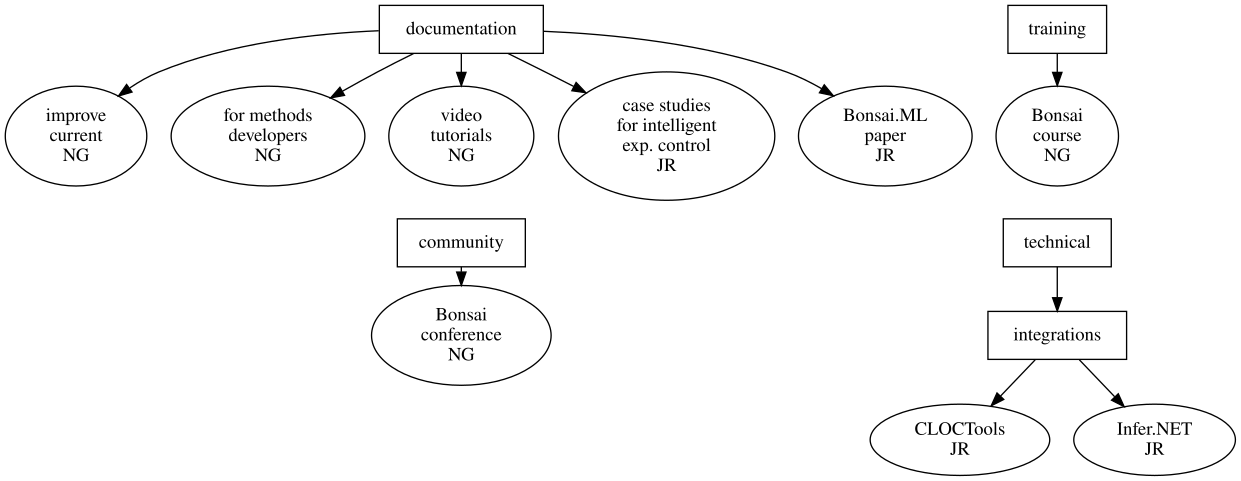
\includegraphics[width=6in]{activitiesGraphs/activities_larger.png}

    \caption{Proposed activities. The initials below each task name indicate
    the responsible team member (JR: Joaquin Rapela, NG: NeuroGEARS Ltd). See
    text for details.}

\end{figure}

\subsection*{Approach}

\subsubsection*{Documentation}

\paragraph{Summary:} Expand Bonsai.ML documentation.

\paragraph{Previous work:} Bonsai.ML already contains detailed
\href{https://bonsai-rx.org/machinelearning/index.html}{documentation} for all
distributed packages. This documentation includes installation instructions,
API listings, and Bonsai working examples that users can copy and paste into
their Bonsai local runtime and execute. We will improve this documentation as
described next.

\paragraph{Future work (responsible team member):}\mbox{}\\
\begin{itemize}

    \item \textbf{Re-structure documentation following the style of
        \href{https://scikit-learn.org/}{scikit-learn} (NG)}. Our current
        documentation lacks accessible statistical explanations of each method
        and clear links between related methods.  We will adopt the style of
        \href{https://scikit-learn.org/}{scikit-learn}, where methods are
        introduced with high-level descriptions, grouped into categories, and
        cross-referenced to practical examples.

    \item\textbf{Provide more examples (NG)} on the application of the already
        integrated ML methods to new types of behavioural and neural data.
        %
        These examples will be similar to the
        \href{https://bonsai-rx.org/machinelearning/examples/README.html}{existing
        ones}, but will be more detailed.
        %
        They should attract to Bonsai.ML a wider group of experimental
        neuroscientists.

    \item\textbf{Include video tutorials (NG)} on the use of the Bonsai.ML
        package, as done in
        \href{https://mark-kramer.github.io/Case-Studies-Python}{Case Studies
        for Neural Data Analysis}, for example
        \href{https://youtu.be/Oj9e2bB3BfI}{here}.

    \item\textbf{Add documentation for methods developers (NG)} as the current
        one is targeted to Bonsai.ML users. For example, we will provide
        detailed instructions to Python developers on how to integrate their
        methods into Bonsai.ML, including explanations about how handles
        Python's global interpreter lock in C\#.

    \item\textbf{Create case studies (JR)} for intelligent experimental control
        in Bonsai, similar to the
        \href{https://mark-kramer.github.io/Case-Studies-Python/intro.html}{case
        studies for neural data analysis in Python}, or those for
        \href{https://mbmlbook.com/index.html}{model based machine learning},
        by our Microsoft collaborators.

    \item\textbf{Publish a first Bonsai.ML paper (JR)} describing its functionality, as
        companion papers substantially increases the adoption of software
        packages \citep{lopesEtAl15,guilbeaultEtAl21}.

\end{itemize}

\noindent\rule{\textwidth}{1pt}
\subsubsection*{Training}
\paragraph{Summary:} Organise a Bonsai course with a dedicated Bonsai.ML module.

\paragraph{Previous work:} Since 2017, NeuroGEARS Ltd has organised at least
two Bonsai courses per year at different universities, and deliver a
one-week-long Bonsai course, hosted at the Sainsbury Wellcome Centre, for
approximately 20 students, targeted to Bonsai users with intermediate
understanding of the language. The structure of the course will be similar to
previous ones (e.g., \href{https://neurogears.org/st-andrews-2024/}{2024 Bonsai
Course at St.~Andrews University}) and is outlined briefly below.

\begin{description}
    \item[Day 1 - Introduction to Bonsai:] What is visual reactive programming? Introduction to Marble diagrams and how to read them. Learning your way around the Bonsai IDE. How to measure and control almost anything with Bonsai. Real-time tracking of colored objects, moving objects and contrasting objects. Measuring behavior using voltages and an Arduino.

    \item[Day 2 - Real-time closed-loop experiments:] Fundamental reactive operators. Data synchronization and measuring closed-loop latency. Conditional effects: triggering a stimulus based on video activity. Continuous feedback: modulate stimulus intensity with speed or distance. Continuous and conditional feedback: closed-loop experiment building blocks. Synchronising asynchronous data streams.

    \item[Day 3 - Operant behavioral tasks:] Sharing observable sequences. Creating dynamic observable sequences with higher-order operators. Modeling trial sequences: states, events, and side-effects. Driving state transitions with external inputs. Best practices for composing complex workflows.

    \item[Day 4 - Machine learning:] Basics of online probabilistic machine learning. Online Bayesian linear regression. Interfacing Bonsai with Python. Linear dynamical systems. Hidden Markov Models. Neural decoding models. Neural latents models.

    \item[Day 5 - Best practices:] How to extend Bonsai with scripting. Reproducible deployment and versioning of experiments. Bonsai hackathon and project presentations. Closing remarks.
\end{description}

\paragraph{Summary:} Organise Bonsai course, with a Bonsai.ML module.

\paragraph{Previous work:} Since 2017, NeuroGEARS Ltd has organised at least
two Bonsai courses per year at different universities, and
\href{https://bonsai-rx.org/learn/}{some of them} can be viewed online. We will
deliver a one-week-long Bonsai course, hosted at the Sainsbury Wellcome Centre,
for approximately 20 students, targeted to Bonsai users with intermediate
understanding of the language. The structure of the course will be similar to
previous ones (e.g., \href{https://neurogears.org/st-andrews-2024/}{2024 Bonsai
Course at St.~Andrews University}).

\paragraph{Outputs:} course delivery, online course material (including lecture
slides, worksheets and video recordings).

\paragraph{Responsible team members:} GL, JR.

\noindent\rule{\textwidth}{1pt}
\subsubsection*{Integrations}

\subsubsection*{Probabilistic programming: Infer.NET}

\paragraph{Background:} Most of the probabilistic models currently integrated
into Bonsai are implemented in Python. These serve as excellent demonstrations
of how Python applications can connect to the Bonsai ecosystem, and they are
central to our aim of attracting Python developers to contribute to Bonsai.ML.
%
However, Python implementations are substantially slower than equivalent C\#
code. For demanding real-time applications, C\# implementations are preferable,
especially when expressed in a probabilistic programming language (PPL).

In addition, the existing Python and C\# implementations of probabilistic
models (e.g., linear dynamical systems, hidden Markov models, Bayesian linear
regression — see
\href{https://bonsai-rx.org/machinelearning/examples/README.html}{examples})
are relatively complex and heterogeneous, in the sense that the implementation
of learning and inference in linear dynamical systems is non-trivial and has
little in common with the implementation of learning and inference in Bayesian
linear regression or in hidden Markov models.
%
In contrast, implementations in a C\# PPL would be much simpler, since PPLs
abstract from their users the complexities of their inference algorithms,
leading to sophisticated inferential methods implemented in a few lines of
code.
%
Also, thanks to this abstraction, implementations of different probabilistic
models in PPLs are substantially more homogeneous in PPLs than in general
purpose ones.

Currently, when we decide to incorporate a new probabilistic model into
Bonsai.ML, we need to implement the learning and inference algorithms for the
specific model, which is generally quite complex and time consuming.
%
In contrast, implementing a new probabilistic model in a PPL only requires the
specification of how the model generates observations, without the
need of specific learning or inference algorithms.
%
Thus, integrating a PPL into Bonsai.ML would greatly simplify the addition of
new probabilistic models to the language.

Fortunately, C\# has an excellent PPL:
\href{https://dotnet.github.io/infer/}{Infer.NET}, developed at Microsoft
Research Cambridge since 2004, used in
\href{https://dotnet.github.io/infer/papers.html}{hundreds of papers}, and
\href{https://www.microsoft.com/en-us/research/blog/the-microsoft-infer-net-machine-learning-framework-goes-open-source/}{open-sourced
in 2018}.  Infer.NET uses deterministic approximate inference, enabling fast
and scalable solutions. For
\href{https://www.microsoft.com/en-us/research/blog/the-microsoft-infer-net-machine-learning-framework-goes-open-source/}{example},
it has powered systems that extract knowledge from billions of web pages
(petabyte-scale data) — the kind of scalability critical for real-time
inference in Bonsai.

\paragraph{Previous work:} Our Microsoft collaborator, Dr.~Tom Minka, invented
a seminal algorithm for inference in graphical models, the Expectation
Propagation algorithm~\citep{minka01}, and is the lead developer of Infer.NET.
Please refer to his letter of support.

\paragraph{Tasks:}\mbox{}\\

\begin{description}

    \item[in\_learn:] the responsible team member is skilled in probabilistic
        programming, but not in Infer.NET. He will invest two weeks in learning
        well the language.

    \item[in\_OBLR:]  Implement in Infer.NET the Online Bayesian Linear
        Regression model, currently implemented in C\# in Bonsai.ML. Develop
        test cases to check that the output of the Infer.Net and previous C\#
        implementations are equal.

    \item[in\_LDS:] Implement in Infer.NET the Linear Dynamical Systems model,
        currently implemented in Python. Develop test cases to check that the
        output of the Infer.Net and previous Python implementations are equal.

    \item[in\_HMM:] Implement in Infer.NET the Hidden Markov Model, currently
        implemented in Python. Develop test cases to check that the output of
        the Infer.Net and previous Python implementations are equal.

    \item[in\_PPdecoder:] Implement in Infer.NET the Point Process Decoding
        model, currently implemented in Python. Develop test cases to check
        that the output of the Infer.Net and previous Python implementations
        are equal.

    \item[in\_docs:] For each of the models integrated above, we will add
        extensive documentation explaining how the models were implemented in
        Infer.NET. The aim is to enable Bonsai.ML users to learn from these
        examples and apply the same principles to build and perform inference
        on their own custom probabilistic models, beyond the ones provided in
        Bonsai.ML-Infer.NET.

\end{description}

\paragraph{Impact:}
This integration will accelerate
inference, simplify and standardise inference programs, and empower Bonsai
users to create new probabilistic models and inference algorithms with just a
few lines of code. Consequently, this activity will drastically improve the
maintainability of the software and facilitate the incorporation of new
probabilistic functionality to the Bonsai ecosystem.

\paragraph{Milestones and Indicators:}\mbox{}\\

\begin{description}

    \item[in\_m1:] OBLR implemented in Bonsai.ML.Infer.NET.

    \item[in\_i1:] Package Bonsai.ML.Infer.NET.OBLR published in nuget.org.

    \item[in\_m2:] LDS implemented in Bonsai.ML.Infer.NET.

    \item[in\_i2:] Package Bonsai.ML.Infer.NET.LDS published in nuget.org.

    \item[in\_m3:] HMM implemented in Bonsai.ML.Infer.NET.

    \item[in\_i3:] Package Bonsai.ML.Infer.NET.HMM published in nuget.org.

    \item[in\_m4:] Point Process Decoder implemented in Bonsai.ML.Infer.NET

    \item[in\_i4:] Package Bonsai.ML.Infer.NET.PP.decoder published in
        nuget.org.

    \item[in\_m5:] Detailed documentation added to all nuget packages above.

    \item[in\_i5:] Eetailed documentation available in the above nuget
        packages.

    \item[in\_m6:] Bonsai.ML.Infer.NET.* packages published.
    \item[in\_i6:] Packages Bonsai.ML.Infer.NET.* available in nuget.org.

\end{description}

\paragraph{Responsible team member:} JR.

\subsubsection*{Closed-loop optogenetic control tools: CLOCTools}

\paragraph{Background:} Closed-loop neural control represents a transformative
advance in neuroscience:  rather than delivering stimulation at fixed,
open-loop schedules, it enables precisely timed interventions based on ongoing
brain and behavioural activity. This paradigm allows researchers to move beyond
observing correlations to  directly testing causal mechanisms of neural
dynamics, plasticity, and behaviour. Critically, closed-loop stimulation has
already proved transformative in the  clinic, for example in deep brain
stimulation for Parkinson’s disease and  epilepsy, while its extension to other
disorders (e.g. depression, obsessive  compulsive disorder) remains an active
area of research. Despite this promise, widespread adoption has been limited
by the lack of accessible, well-engineered,  and sustainable software
frameworks for real-time experimental control.

Prof.~Garrett Stanley (Georgia Tech and Emory University, US) is a pioneer in
closed-loop neuroscience, having developed groundbreaking methods that combine
real-time neural control with systems neuroscience. He recently contacted us to
explore integrating their existing
\href{https://cloctools.github.io/}{CLOCTools}, originally implemented in
RTXI/C++, into Bonsai.ML.  This represents a unique opportunity: Bonsai already
excels at real-time closed-loop control in behavioural experiments, and
extending it to include state-of-the-art closed-loop neural control will
position the platform as the first sustainable, general-purpose framework for
both levels of experimentation.

An important reason for the poor uptake of closed-loop methods in neuroscience
could be that existing implementations are often ad hoc, difficult to install
or  extend, and not integrated with software for experimental control. By
providing Bonsai users with accessible, open-source, and sustainably engineered
tools for closed-loop control, we will directly address this barrier and enable
a new type of experimentation where researchers can both read and write the
neural code in real time. This will accelerate discovery across both basic and
translational neuroscience.

\paragraph{Previous work:} Members of Prof.~Stanley’s lab have already
prototyped some of their closed-loop control methods in Bonsai using our
\href{https://bonsai-rx.org/python-scripting/}{Python scripting interface}.
Please refer to the repositories in the
\href{https://github.com/ndac-bonsai}{ndcac-bonsai} organisation containing
these prototypes (ndac stands for neural dynamic adaptive control).

\paragraph{Tasks:}\mbox{}\\

\begin{description}

    \item[hsc\_C\#\_Infer.NET:] Implement the Python package Hybrid System
        Control in C\#.
	%
        Runtime performance is critical for the control of neural system, and a
        C\# implementation should be much faster than a Python one.
	%
        The Python implementation uses the ssm Python library to perform
        inference in linear dynamical systems. Instead, we will
        use Bonsai.ML.Infer.NET.LDS previously developed. (4 weeks)

    \item[hsc\_test\_cases:] Develop test cases for the C\# implementation of
        HybridSystemControl, comparing is functionality with that of the
        original Python implementation. Fix any resulting problem. (2 weeks)

    \item[hsc\_bonsai\_integration:] Integrate the C\# implementation of HybridSystemControl
        into Bonsai, generating the Bonsai.ML.HybridSystemControl package.  (2
        weeks)

    \item[hsc\_eval\_synthetic:] Evaluate the package
        Bonsai.ML.HybridSystemControl with synthetic data and fix problems.
        These evaluation will focus on testing if the package can achieve the
        real-time latency constraints required in neuroscience applications. (2
        weeks)

    \item[hsc\_eval\_exp:] Assist the laboratory of Prof.~Stanely in
        testing Bonsai.ML.HybridSystemControl with experimental data, and
        address problems. (4 weeks)

    \item[hsc\_docs:] Add documentation to Bonsai.ML.HybridSystemControl, in a
        similar style as the new documentation of other Bonsai.ML packages. (3
        weeks)

    \item[hsc\_release:] Release the Bonsai.ML.HybridSystemControl package. (1
        week)

\end{description}

\paragraph{Milestones and Indicators:}\mbox{}\\

\begin{description}

    \item[hsc\_m1:] Package HybridSystemControl implemented in C\#.

    \item[hsc\_i1:] Package HybridSystemControl published in nuget.org.

    \item[hsc\_m2:] Test cases added  to HybridSystemControl.

    \item[hsc\_i2:] Test cases available in nuget package HybridSystemControl.

    \item[hsc\_m3:] Package Bonsai.ML.HybridSystemControl created.

    \item[hsc\_i3:] Package Bonsai.ML.HybridSystemControl available in GitHub
        repository.

    \item[hsc\_m4:] Package Bonsai.ML.HybridSystemControl evaluated with
        synthetic data.

    \item[hsc\_i4:] Workflows demonstrating the correct functionality with
        syntetic data of the package Bonsai.ML.HybridSystemControl available in
        GitHub repository.

    \item[hsc\_m5:] Functionality of Bonsai.ML.HybridSystemControl demonstrated
        with experimental data.

    \item[hsc\_i5:] Experimental evidence available in GitHub repository demonstrating that the package
        Bonsai.ML.HybridSystemControl succeeded holding the firing rate of a
        single neuron in the thalamus at a steady level with optogenetic
        inputs, while a mouse was visually stimulated.

    \item[hsc\_m6:] Documentation added to Bonsai.ML.HybridSystemControl.

    \item[hsc\_i6:] API documentation, examples and tutorials available in
        GitHub repository.

    \item[hsc\_m7:] Package Bonsai.ML.HybridSystemControl released.

    \item[hsc\_i7:] Bonsai.ML.HybridSystemControl available in nuget.org.

\end{description}

\paragraph{Responsible team members:} JR

\noindent\rule{\textwidth}{1pt}
\subsubsection*{Governance}

We will create a Bonsai.ML steering committee that will be responsible for
approving project milestones and advise us on building a long-term development
roadmap for Bonsai.ML.
%
Responding to guidance and feedback from the steering committee ensures
Bonsai.ML addressed pressing neuroscience needs on an international scale.

Several renowned experimental and computational neuroscientists around the
world are heavily invested in Bonsai, are very interested in adding ML
functionality to their Bonsai workflows, and have agreed to join the Bonsai.ML
steering committee. We list them below.

\begin{description}

    \item[Prof.~Garrett Stanley,] leader of the Laboratory for the Control of
        Neural Systems, Georgia Tech, US. Expert on close-loop control of
        neurophysiological systems. He contacted us to migrate to Bonsai
        a package for real-time cortical state estimation and the CLOCTools
        referred above, both originally written in C++/RTXI.

    \item[Prof.~Aman Saleem,] director of the Saleem Lab at the Institute for
        Behavioural Neuroscience, University College London. Prof.~Saleem is the
        author of \href{https://bonvision.github.io/}{Bon-Vision}, a software
        package that creates and controls visual environments in close loop,
        built on top of Bonsai.

    \item[Prof.~Josh Siegle,] senior scientist and lead of the
        electrophysiology group at the Allen Institute for Neural Dynamics. He
        leads the development of Open Ephys GUI, which is tightly integrated
        with Bonsai.

    \item[Prof.~Ken Harris,] co-director of the Cortexlab, University College
        London, and founding director of the International Brain Laboratory,
        that uses Bonsai for reproducible experimental control across 22
        laboratories around the world.

    \item[Prof.~Athena Akrami,] director of the Learning, Inference and Memory
        Lab, at the SWC, that uses Bonsai extensively for the control of
        complex rodent experiments in her lab.

\end{description}

\noindent\rule{\textwidth}{1pt}
\subsection*{Management}

We will conduct management activities at different frequencies:

\begin{description}

    \item[Twice a year:] we will convene the steering committee. Two weeks in
        advance of each meeting, we will circulate a progress report
        summarising achieved milestones, proposed future activities, and the
        most recent version of the Bonsai.ML long-term roadmap.
        %
        The steering committee will review the report, endorse completed
        milestones, and provide feedback or suggestions on planned activities.
        %
        Based on project progress and committee input, we will revise the
        long-term roadmap, ensuring that Bonsai.ML development remains aligned
        with community needs and strategic goals.
        %
        Minutes and key decisions from these meetings will be documented and,
        where possible, shared with the Research Software Maintenance Fund
        through appropriate reporting channels.

    \item[Every month:] we will hold meetings between the project lead, the
        project co-lead, the RSE, and the external project co-lead, to evaluate
        the project progress.

    \item[Weekly:] as has been our practice since the start of the Bonsai.ML
        project, the RSEs will meet with the external project co-lead to
        discuss issues that appeared during the week, review activities for the
        following week, and adjust project directions.

\end{description}

Meetings with collaborators will be arranged as needed.
%
At the SWC, GCNU and NG we are experimental and computational neuroscientists
with successful collaborative experience, and we have no doubt that the
proposed collaborations will be of the same kind,
%
specially since we have successfully interacted in the past with most of the
propose collaborators.
%
Please refer to their letters of support.


\subsection{Workplan (optional)}

\begin{instruction}
You may choose to upload a one page document such as a Gantt chart to help illustrate timing of and links among the activities.
\end{instruction}

\begin{center}
    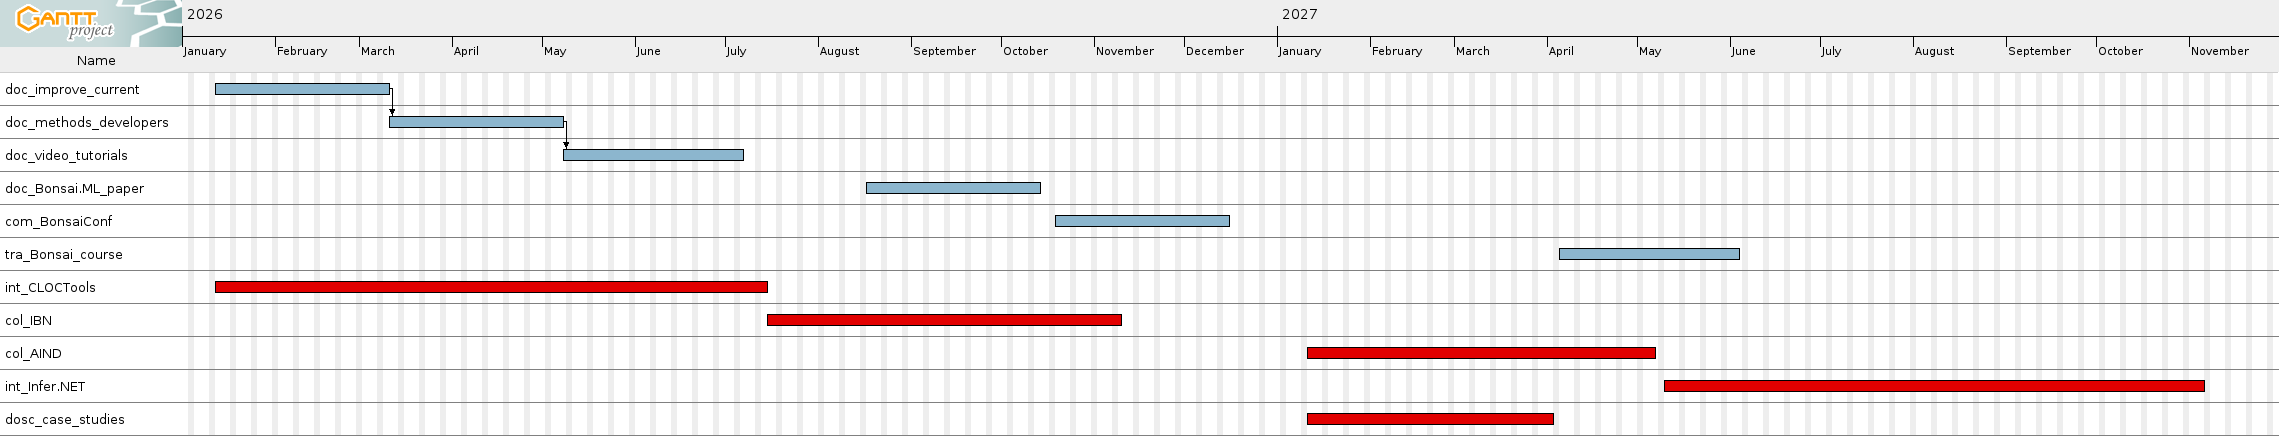
\includegraphics[width=6.5in]{figures/ganttChart1.png}
\end{center}

\pagebreak

\section{Capability to deliver (1000 words)}

\begin{instruction}
Provide evidence of how you and your team have:

    \begin{itemize}
        \item the relevant experience (appropriate to career stage) to deliver the objectives
        \item the right balance of skills and expertise to cover the proposed work
        \item the appropriate leadership and management skills to ensure delivery
        \item contributed to developing good practice in your communities
    \end{itemize}

Where applicable, discuss your approach to developing others.

\end{instruction}


\subsection{Relevant Experience}

\paragraph{TMF} is an experimental
neuroscientists and director of the SWC. Research in his laboratory aims to
explain how the brain makes decisions by combining sensory information with
previously learned knowledge.  As the behavioural tasks used in his lab require
complex software-control of data acquisition and data analysis pipelines, he
knows first-hand their crucial importance for driving and enabling
neuroscientific research.

He has published 49 peer-reviewed papers, with an h-index of 35 (calculated by
google scholar).  He is a founding member of the International Brain Laboratory
(IBL et al 2019 Neuron). The Bonsai ecosystem is critical to IBL, as it ensures
that experimental control, stimulus presentation and data acquisition can be
identically reproduced across all participating labs in UK, Europe and USA (IBL
et al 2021, eLife)

\paragraph{MS} is a computational neuroscientists and director of the Gatsby
Unit. He has authored over 100 peer-reviewed scientific papers, with an h-index
(computed by Google scholar) of 47. A substantial component of his research
focuses on the development of advance machine-learning based tools for
neuroscience research.

Beginning around 2005, his group published a series of new neuroinformatics
tools designed to characterise and understand population-scale activity using
the large-scale multielectrode recording methods being developed. These papers
provided the backbone for a new analytic approach that is now being employed
and extended by systems neuroscience laboratories worldwide.
%
Key papers include Yu et al., 2006, Yu et al., 2009 and Macke et al., 2011,
Duncker et al., 2019, Rutten et al., 2020 and Soulat et al., 2021.
%
A central component of the current proposal is to disseminate this approach
(and others) already available within Bonsai, easing its adoption by a wider
group of laboratories that lack in-house informatics expertise.

\paragraph{GL} is the creator of Bonsai and has ample experience in software
engineering, holding a Licentiate degree in Computer Science from NOVA
University Lisbon, and having worked between 2006 and 2010 at the NOVA CENTRIA
Artificial Intelligence laboratory, and at YDreams, where he was leading a team
developing a ground-breaking engine for Augmented Reality.

Transitioning into his neuroscience PhD at the Champalimaud Foundation, he
created the Bonsai visual programming language to run his PhD experiments,
which then led him to managing a software development company serving thousands
of users and collaborating with leading universities and research centres
around the world.

\paragraph{JR} specializes in
signal processing and machine learning, with applications to understanding
brain function (Rapela et al., 2006, Rapela et al., 2010, Rapela et al., 2018
and Rapela et al., 2019).

He has extensive software development expertise, holding a Master’s degree in
Computer Science and industry experience at IBM Argentina and the IBM Almaden
Research Center, US.
%
He joined the Gatsby Computational Neuroscience Unit in 2019 as a Research
Engineer Fellow.
%
He is the lead developer of \href{https://github.com/joacorapela/svGPFA}{Sparse
Variational Gaussian Process Factor Analysis (svGPFA)}, and has openly released
several other machine learning packages including linear dynamical systems in
\href{https://github.com/joacorapela/ssm}{Python} and
\href{https://github.com/joacorapela/kalmanFilter}{R},
\href{https://github.com/joacorapela/hiddenMarkovModels}{Hidden Markov Models}
in R, and
\href{https://github.com/joacorapela/bayesianLinearRegression}{Bayesian Linear
Regression} in Python.

JR played a leading role in securing the BBSRC grant that funded the
creation of Bonsai.ML and has led its development since the project’s
inception. He also played a central role in preparing the current proposal.


\subsection{Balance of Skills and Expertise}

Our team has the required expertise, at the leadership and development levels,
in machine learning (MS, JR, NG), software development (GL, JR, NG), neuroscience
(TMF, MS, GL, JR, NG) and experimental control (GL, NG).

Our expertise is complemented by that of world-class project partners in
close-loop neural control (Prof.~Garrett Stanley) and probabilistic programming
(Dr.~Tom Minka), required for the integration activities; and that in
high-channel-count electrophysiological recordings (Dr.~Josh Siegle) and vision
and navigation (Prof.~Aman Saleem), required for the collaborative activities.
Please refer to their letters of support.

\subsection{Leadership and Management Skills}

\paragraph{TMF} is the Director of the Sainsbury Wellcome Centre (SWC) at
University College London. He is responsible for setting the Centre’s strategic
and scientific direction, which currently comprises 12 experimental labs. In
addition, he has line management responsibilities for the Executive Team,
several members of the SWC Faculty, and numerous scientific and administrative
support staff.

\paragraph{MS} has been Director of the Gatsby Computational
Neuroscience Unit since 2017, leading strategy in research and teaching. He has
created two new roles to support and develop new strategy, and has recruited
two new members of faculty who.  As Director, he sits in the Executive
Leadership Committee of the Faculty of Life Sciences at UCL.

\paragraph{GL} is the Founder and Director of NeuroGEARS since 2017, where he has led a diverse team of scientists, engineers and artists in the development of novel experimental platforms across multiple model organisms. He has also directly contributed in the organisation and teaching of Bonsai for neuroscience experimentation worldwide, and was part of the creation of the Neuronauts educational outreach programme. Currently, NeuroGEARS employs 8 scientists and engineers across the UK, US and Portugal.

\paragraph{JR} has lead a small team of RSEs in the
creation of the Bonsai.ML package since 2023.

\subsection{Contribution to Developing Good Practice in Communities}

GL has contributed as TA, faculty, and organizer, to numerous experimental neuroscience and Bonsai programming courses at the PhD level. In these courses, students learn about software development and science instrumentation best practices, including version control, testing, reusable software, data formats, and quality control of scientific data from acquisition to analysis.

Materials developed throughout these courses, which are shared openly under open-source licenses, now form the basis of best practices and standards across the Bonsai user and neuroscience communities worldwide.

GL is an active upstream contributor to many open-source projects, and actively promotes open technical discussions. At the \href{https://github.com/orgs/bonsai-rx/discussions}{Bonsai discussions} forum, scientists and engineers can openly present their problem, discuss their technical solutions in detail, and assimilate best
Bonsai practices, which are then used to inspire future open-source course materials, and to improve software development and documentation.

JR has contributed to software carpentry courses.


\subsection{Developing others}

\paragraph{TMF} has led a laboratory since 2008. He has
successfully supervised 10 MA students, 7 PhD students, and 12 postdoctoral
scholars.

\paragraph{MS} has supervised a total of 14 PhD students and
14 postdoctoral fellows.

\paragraph{GL} has supervised and trained over 10 scientists and engineers at NeuroGEARS since 2017, and co-supervised 2 iCASE studentships in collaboration with UCL faculty.

\paragraph{JR} co-mentored a masters, two undergraduate
students and is advising an RSE in machine learning methods development.


\pagebreak

\section{Project partners}

\begin{instruction}

A project partner is a collaborating organisation that plays an integral role in the proposed work. You should describe the nature of this support in the Approach section of your application.

Project partners contribute to the delivery of the project and should not normally request funding from the grant. However, travel and subsistence costs incurred by the lead organisation to enable project partner involvement may be included—these must be fully justified in the Resources section.

You cannot include an individual as an applicant (i.e., project lead, co-lead, or any Core Team role) if they, or their organisation, are named as the project partner contact.

All project partners must be listed as contributors below, and a letter of support for each must be uploaded as a single combined PDF.

\end{instruction}

\subsection{Letter(s) of Support (optional)}

\pagebreak

\section{Resources}

\begin{instruction}

Please provide details of the funding requested.

Use the breakdown categories listed in this section, and discuss the main resource requirements.

You will also need to upload a consolidated budget from the lead organisation using a standard FEC costing format.

\end{instruction}

\subsection{Justification of resources (1000 words)}

\begin{instruction}

Justify the application’s more costly resources, in particular:

\begin{itemize}
    \item any staff costs
    \item significant costs related to collaboration or community engagement
    \item any consumables beyond typical requirements
    \item infrastructure costs
    \item all resources that have been costed as ‘Exceptions’
\end{itemize}

You do not need to justify Estates and Indirect costs.

We are not looking for a detailed breakdown of each cost, but want you to demonstrate how the resources you are applying for are comprehensive, appropriate and justified, and represent the optimal use of resources to achieve the intended outcomes.

\end{instruction}

\paragraph{Staff costs:} cover the salary of two research software engineers working on the project.

\paragraph{Community engagement:} The directly incurred \texttt{Other costs} cover the costs of one training curse and one developers conference. These cost only cover food expenses, as the venue is provided free of charge by the Sainsbury Wellcome Centre.

\paragraph{Cash contributions:}
NeuroGEARS will contribute £5,733.60 in cash towards salary support for one RSE.

\paragraph{In-kind contributions:}
NeuroGEARS will provide in-kind contributions valued at £100,000, including:

\begin{enumerate}
    \item Supporting the organisation of a Bonsai course, including a Bonsai.ML module, and providing instructors for its delivery.

    \item Supporting the organisation of the 2026 Bonsai Development Conference, including a Bonsai.ML session, and providing instructors for its delivery.

    \item Organising and deploying a Bonsai booth, including a Bonsai.ML exhibit, at the 2025 Society for Neuroscience Annual Meeting, similar to that deployed in 2024.

    \item Delivering Bonsai and Bonsai.ML lectures at the annual
    \href{https://github.com/joacorapela/statNeuro2025}{Sainsbury Wellcome Centre Statistical Neuroscience course}.

    \item Contributing director time to the Bonsai.ML weekly meetings.

    \item Providing Bonsai technical support to members of the Bonsai.ML team.
\end{enumerate}

\subsection{Total funding requested:} £283,384.02

\subsection{Directly incurred - Staff:} £130,539.22

\subsection{Directly incurred - Travel and Subsistence:} £0.0

\subsection{Directly incurred - Other:} £13,600

\subsection{Directly allocated - Staff:} £0.0

\subsection{Directly allocated - Estates:} £26,100.80

\subsection{Directly allocated - Other:} £0.0

\subsection{Indirects:} £113.144

\subsection{Exceptions:} £0.0

\bibliographystyle{apalike}
\bibliography{bonsai,longDurationExperimentation,physiology,optogenetics,closeLoopControlOfNeuralActivity,latentsVariablesModels,messagePassing,neuralControl}

\end{document}
